% basic nastaveni
\documentclass[12pt]{article}
\setlength{\parindent}{0pt}
\setlength{\parskip}{1em}
\usepackage[utf8]{inputenc}
\usepackage[czech]{babel}
\usepackage[T1]{fontenc}
\usepackage{graphics}
\usepackage{caption}
\usepackage{hyperref}
\usepackage{xcolor}
\usepackage{float}

% matematicke package
\usepackage{amsmath}
\usepackage{amsfonts}
\usepackage{amssymb}
\usepackage{geometry}
\geometry{margin=2.5cm}
\usepackage{pgfplots}
\pgfplotsset{compat=1.18}
\usepackage{mathrsfs}

\title{Maturitní otázka číslo 7: Goniometrie a trigonometrie}
\author{}
\date{}

\begin{document}
\maketitle
\subsection*{Goniometrické funkce}
Goniometrické funkce jsou takzvaně transcendentní funkce, jejichž hodnoty nelze vypočítat pouze s
využitím algebraických operací. Goniometrické funkce mají jako vstupní hodnotu velikost úhlu. Pro
naše chápání pro středoškolskou matematiku se goniometrické funkce definují pomocí pravoúhlého
trojúhelníku nebo jednotkové kružnice.
\begin{figure}[htbp]
    \centering 
    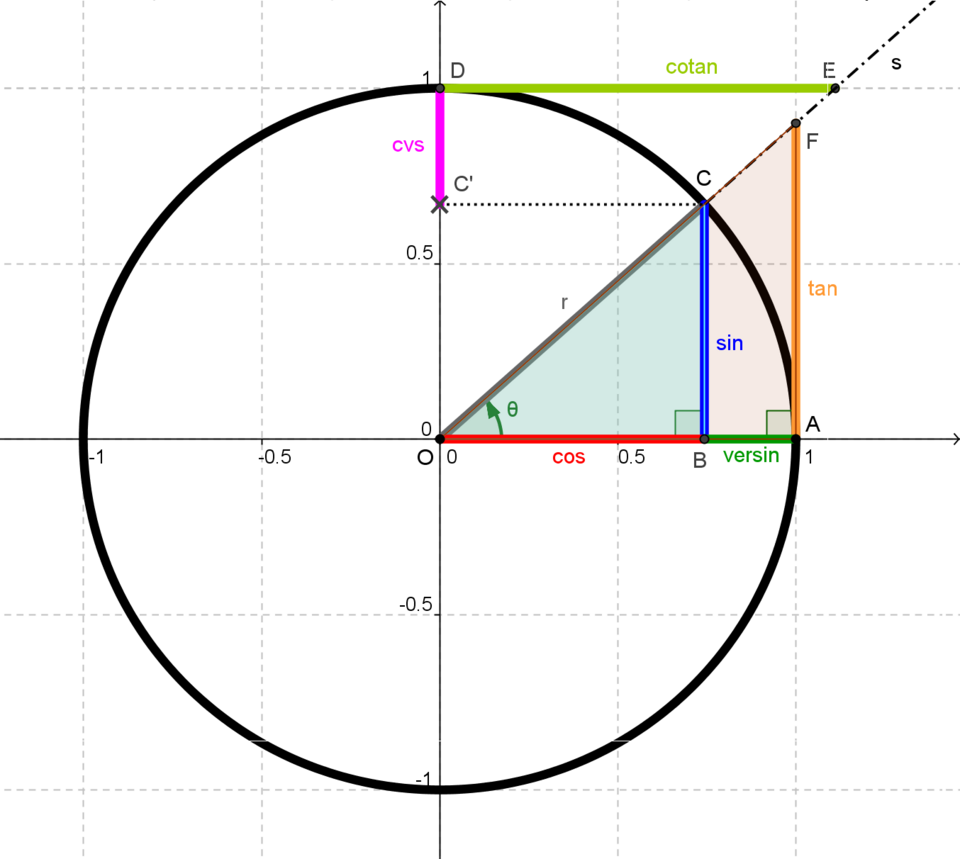
\includegraphics[width=0.5\textwidth]{pictures/jednotkova_kruznice.png}
    \caption*{}
\end{figure}
\subsubsection*{Sinus}
Sinus je v pravoúhlém trojúhelníku definován jako poměr protilehlé odvěsny k přeponě $\sin(\alpha)
= \frac{\text{protilehlá}}{\text{přepona}}$. Definiční obor je $D(f) = \mathbb{R}$ a obor hodnot je
$H(f) = \langle -1, 1 \rangle$. Funkce je lichá a periodická s periodou $2 \pi$ neboli $360^\circ$.
Grafu se říká sinusoida.
\begin{figure}[H]
    \centering 
    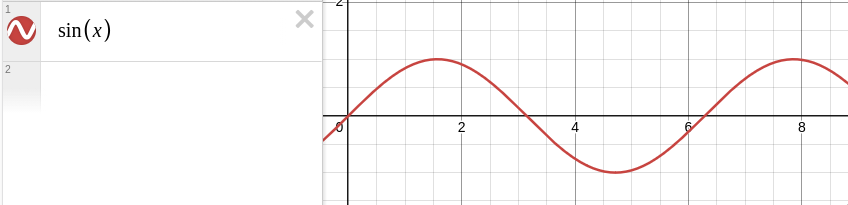
\includegraphics[width=0.7\textwidth]{pictures/sinus.png}
    \caption*{}
\end{figure}
\subsubsection*{Cosinus}
Cosinus je v pravoúhlém trojúhelníku definován jako poměr přilehlé odvěsny k přeponě $\cos(\alpha)
= \frac{\text{přilehlá}}{\text{přepona}}$. Definiční obor je $D(f) = \mathbb{R}$ a obor hodnot je
$H(f) = \langle -1, 1 \rangle$. Funkce je sudá a periodická s periodou $2 \pi$ neboli $360^\circ$.
Grafu se říká cosinusoida.
\begin{figure}[H]
    \centering 
    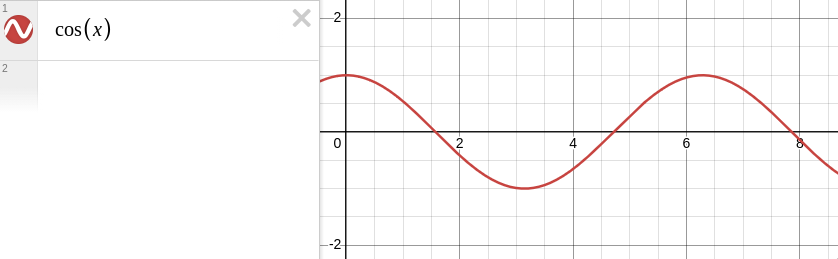
\includegraphics[width=0.7\textwidth]{pictures/cosinus.png}
    \caption*{}
\end{figure}
\subsubsection*{Tangens}
Tangens je v pravoúhlém trojúhelníku definován jako poměr protilehlé odvěsny k přilehlé odvěsně
$\tan(\alpha) = \frac{\text{protilehlá}}{\text{přilehlá}}$ a také platí $\tan(\alpha) =
\frac{\sin(\alpha)}{\cos(\alpha)}$. Definiční obor je $D(f) = \mathbb{R} \setminus \{\frac{\pi}{2} +
k \pi \}, k \in \mathbb{Z}$ a obor hodnot je $H(f) = \mathbb{R}$. Funkce je lichá, rostoucí a
periodická s periodou $\pi$ neboli $180^\circ$. Grafu se říká tangentoida.

\begin{figure}[H]
    \centering 
    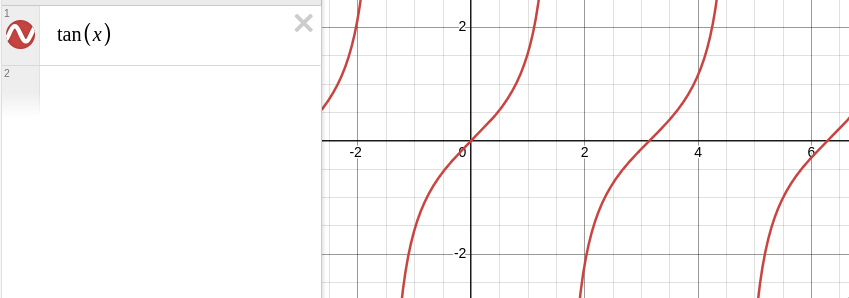
\includegraphics[width=0.7\textwidth]{pictures/tangens.png}
    \caption*{}
\end{figure}

\subsubsection*{Cotangens}
Cotangens je v pravoúhlém trojúhelníku definován jako poměr přilehlé odvěsny k protilehlé odvěsně
$\tan(\alpha) = \frac{\text{přilehlá}}{\text{protilehlá}}$ a také platí $\cot(\alpha) =
\frac{\cos(\alpha)}{\sin(\alpha)}$. Definiční obor je $D(f) = \mathbb{R} \setminus \{k \pi \}, k \in
\mathbb{Z}$ a obor hodnot je $H(f) = \mathbb{R}$. Funkce je lichá, klesající a periodická s
periodou $\pi$ neboli $180^\circ$. Grafu se říká cotangentoida.

\begin{figure}[H]
    \centering 
    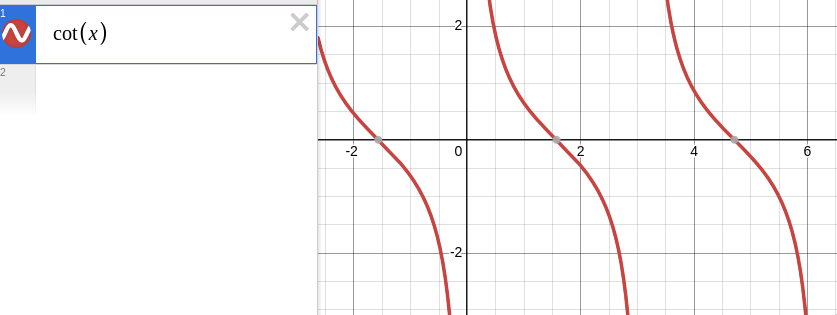
\includegraphics[width=0.7\textwidth]{pictures/cotangens.png}
    \caption*{}
\end{figure}
\subsubsection*{Vzorečky}
Pro goniometrické funkce existuje velké množnství různých vzorců, které se vyskytují například v
tabulkách.

\subsection*{Sinová věta}
Sinova věta platí pro všechny trojúhelníky a říká nám, že poměr délky strany a sinu protilehlého
úhlu je v trojúhelníku konstantní $\frac{a}{\sin(\alpha)} = \frac{b}{\sin(\beta)} = \frac{c}{\sin(
\gamma)}$. Tento poměr je také roven průměru kružnice opsané daného trojúhelníku $\frac{a}
{\sin(\alpha)} = 2r$.
\subsection*{Cosinová věta}
Cosinová věta je zobecněná pythagorova věta pro trojúhelníky, které nemusí mít pravý úhel.
Platí $a^2 = b^2 + c^2 - 2bc \cdot \cos \alpha$. Vzorec existuje pro všechny strany, tedy také platí
$b^2 = a^2 + c^2 - 2ac \cdot \cos \beta$ a $c^2 = a^2 + b^2 - 2ab \cdot \cos \gamma$. Pokud bychom
používali tuto větu pro odvěsnu pravoúhlého trojúhelníku, $\cos(90^\circ)$ je roven nule, a zbyde nám
známá Pythagorova věta.
\end{document}
